%%%%%%%%%%%%%%%%%%%%%%%%%%%%%%%%%%%%%%%%%%%%%%%%%%%%%%%%%%%%%%%%%%%%%%%%%%%%%%%%
%%%%%%%%%%%%%%%%%%   Vorlage für eine Abschlussarbeit   %%%%%%%%%%%%%%%%%%%%%%%%
%%%%%%%%%%%%%%%%%%%%%%%%%%%%%%%%%%%%%%%%%%%%%%%%%%%%%%%%%%%%%%%%%%%%%%%%%%%%%%%%

% Erstellt von Maximilian Nöthe, <maximilian.noethe@tu-dortmund.de>
% ausgelegt für lualatex und Biblatex mit biber

% Kompilieren mit
% latexmk --lualatex --output-directory=build thesis.tex
% oder einfach mit:
% make

\documentclass[
  tucolor,       % remove for less green,
  parskip=full,  % new paragraphs start with half line vertical space
  open=any,      % chapters start on both odd and even pages
  cleardoublepage=plain,  % no header/footer on blank pages
]{tudothesis}

\setlength{\parindent}{0pt}

\usepackage{scrlayer-scrpage}
% Clear any previous header/footer settings
\clearpairofpagestyles

% Set the footer to the bottom right
\ohead[\thepage]{\thepage}

% Ensure page numbers are not in italics
\setkomafont{pagefoot}{\normalfont}

% Warning, if another latex run is needed
\usepackage[aux]{rerunfilecheck}

% just list chapters and sections in the toc, not subsections or smaller
\setcounter{tocdepth}{2}

%------------------------------------------------------------------------------
%------------------------------ Fonts, Unicode, Language ----------------------
%------------------------------------------------------------------------------
\usepackage{fontspec}
\defaultfontfeatures{Ligatures=TeX}  % -- becomes en-dash etc.

% load english (for abstract) and ngerman language
% the main language has to come last
% Use line below if thesis is written in german
% \usepackage[american, ngerman]{babel}
% Use line below if thesis is written in english
\usepackage[ngerman, american]{babel}

% intelligent quotation marks, language and nesting sensitive
\usepackage[autostyle]{csquotes}

% microtypographical features, makes the text look nicer on the small scale
\usepackage{microtype}

%------------------------------------------------------------------------------
%------------------------ Math Packages and settings --------------------------
%------------------------------------------------------------------------------

\usepackage{amsmath}
\usepackage{amssymb}
\usepackage{mathtools}

% Enable Unicode-Math and follow the ISO-Standards for typesetting math
\usepackage[
  math-style=ISO,
  bold-style=ISO,
  sans-style=italic,
  nabla=upright,
  partial=upright,
  warnings-off={mathtools-colon,mathtools-overbracket}, % suppress some unnecessary warnings
]{unicode-math}
\setmathfont{Latin Modern Math}

% nice, small fracs for the text with \sfrac{}{}
\usepackage{xfrac}


%------------------------------------------------------------------------------
%---------------------------- Numbers and Units -------------------------------
%------------------------------------------------------------------------------

\usepackage[
  locale=DE,
  separate-uncertainty=true,
  per-mode=symbol-or-fraction,
]{siunitx}

\addto\extrasngerman{\sisetup{locale = DE}}
\addto\extrasenglish{\sisetup{locale = US}}

%------------------------------------------------------------------------------
%-------------------------------- tables  -------------------------------------
%------------------------------------------------------------------------------

\usepackage{booktabs}       % \toprule, \midrule, \bottomrule, etc

%------------------------------------------------------------------------------
%-------------------------------- graphics -------------------------------------
%------------------------------------------------------------------------------

\usepackage{graphicx}
% currently broken
% \usepackage{grffile}

% allow figures to be placed in the running text by default:
\usepackage{scrhack}
\usepackage{float}
\floatplacement{figure}{htbp}
\floatplacement{table}{htbp}

% keep figures and tables in the section
\usepackage[section, below]{placeins}

% allows to include PDFs as full pages
\usepackage{pdfpages}

% Allows for figures wraped with text
\usepackage{wrapfig}

% Set the PDF Version of this document to 1.7 (1.4 is the current default)
% This is needed so that PDFs with Version >1.5 can be included
\pdfvariable minorversion=7

%------------------------------------------------------------------------------
%---------------------- customize list environments ---------------------------
%------------------------------------------------------------------------------

\usepackage{enumitem}

%------------------------------------------------------------------------------
%------------------------------ Bibliographie ---------------------------------
%------------------------------------------------------------------------------

\usepackage[
  backend=biber,   % use modern biber backend
  autolang=hyphen, % load hyphenation rules for if language of bibentry is not
                   % german, has to be loaded with \setotherlanguages
                   % in the references.bib use langid={en} for english sources
  sorting=none,
]{biblatex}
\addbibresource{references.bib}  % the bib file to use
\DefineBibliographyStrings{german}{andothers = {{et\,al\adddot}}}  % replace u.a. with et al.


% Last packages, do not change order or insert new packages after these ones
\usepackage[pdfusetitle, unicode, linkbordercolor=tugreen, citebordercolor=tugreen]{hyperref}
\usepackage{bookmark}
\usepackage[shortcuts]{extdash}

%------------------------------------------------------------------------------
%-------------------------    Angaben zur Arbeit   ----------------------------
%------------------------------------------------------------------------------

\author{Akram Aki}
\title{CINIC-10 Source Classifier: Learning to Tell CIFAR from ImageNet}
\date{2025}
\birthplace{Hagen, Germany}
\chair{WG Rhode / Elsässer}
\division{Fakultät Physik}
\thesisclass{Machine Learning for Physicists}
\submissiondate{31. July 2025}
\firstcorrector{Dr.~Carsten~Burgard}
\secondcorrector{Dr.~Cornelius~Grunwald}

% tu logo on top of the titlepage
\titlehead{
\includegraphics[height=1.5cm]{logos/tu-logo.pdf}}

\begin{document}
% BEFORE TOC (e.g., Abstract, Acknowledgements)
\pagenumbering{roman}  % i, ii, iii, ...
\setcounter{page}{1}   % restart from i

%\frontmatter
\maketitle

% Gutachterseite
\makecorrectorpage

% hier beginnt der Vorspann, nummeriert in römischen Zahlen
\thispagestyle{plain}

\section*{Abstract}
The goal of this project was to build a classifier capable of determining whether an image in the CINIC-10 dataset originates from CIFAR-10 or from ImageNet. 
To this end, we analyzed statistical and visual differences between the two domains, including RGB mean values, per-class variance and structural image characteristics.
We tested various machine learning approaches, including Convolutional Neural Networks (CNNs), Multi-Layer Perceptrons (MLPs) as well as classical models like Random Forests. 
In addition to training models, we explored interpretability techniques such as visualizing activation maps and analyzing learned convolutional filters. 
The results show that even without class labels, models can learn to distinguish the source domain of images based on subtle differences in data characteristics.
All code and instructions to reproduce the results are available in the associated GitHub repository~\cite{cinic10-source-classifier}.

\section*{Kurzfassung}
\begin{foreignlanguage}{german}
In diesem Projekt wurde das Ziel verfolgt, einen Klassifikator zu entwickeln, der innerhalb des CINIC-10-Datensatzes erkennen kann, ob ein Bild ursprünglich aus CIFAR-10 oder aus ImageNet 
stammt. Dafür wurden zunächst die Metadaten ausgewertet und visuelle sowie statistische Unterschiede zwischen den beiden Quellen analysiert, z.B. RGB-Mittelwerte, 
Varianz pro Klasse und Strukturmerkmale der Bilder.
Zur Modellentwicklung wurden verschiedene Machine Learning Ansätze getestet, darunter Convolutional Neural Networks (CNNs), Multi-Layer Perceptrons (MLPs) sowie klassische Verfahren wie 
Random Forests.
Neben der Modellierung wurden auch Ansätze zur Interpretation der Modelle verfolgt, etwa durch Visualisierung einzelner Bilder nach durchlauf des Kernel Filters oder 
durch die Visualisierung gelernter Filter. 
Das Projekt zeigt, dass auch ohne explizite Objektklassenunterscheidung Unterschiede in der Datenquelle durch maschinelles Lernen erkannt werden können.
Der vollständige Code sowie eine Anleitung für Basis Einstellungen sind im zugehörigen GitHub-Repository~\cite{cinic10-source-classifier} zu finden.
\end{foreignlanguage}

\newpage 
\tableofcontents

\newpage

% MAIN CONTENT
\pagenumbering{arabic} % 1, 2, 3, ...
\setcounter{page}{1}   % restart from 1

%\mainmatter
% Hier beginnt der Inhalt mit Seite 1 in arabischen Ziffern
\section{Introduction}

The automated classification of visual data is one of the central tasks in modern machine learning. Over the past decade, datasets such as \textbf{CIFAR-10} and \textbf{ImageNet} have played a 
pivotal role in the development and evaluation of deep learning models. These datasets differ not only in resolution and content diversity, but also in how images are collected, 
preprocessed, and labeled. While CIFAR-10 consists of small, uniformly processed images of objects centered against clean backgrounds, ImageNet offers a broader and more varied selection 
of real world scenes.
The \textbf{CINIC-10 dataset} (CINIC = \textit{CINIC Is Not ImageNet or CIFAR}) merges images from CIFAR-10 and downsampled ImageNet into a unified 10-class structure. 
It was primarily created to bridge the gap between the simplicity of CIFAR-10 and the complexity of ImageNet, enabling more robust benchmarking. However, this fusion may also 
introduce domain-specific artifacts, which could prevent certain machine learning approaches from reaching their full potential.
In this project, we explore the question:
\begin{center}
\textbf{\textit{Can a ML model distinguish the original source of an image in CINIC-10?}}
\end{center}
To answer this, we analyzed the dataset at multiple levels. First, we investigated low-level statistical properties, such as per-class RGB channel means and variances, to detect structural 
biases between the two sources. For instance, CIFAR-10 images often appear more ``stock-like'', meaning well-centered, consistently lit, and visually uniform. ImageNet derived images tend 
to be more diverse, naturalistic, and less curated in appearance.
Second, we trained a variety of models, ranging from shallow multi-layer perceptrons to convolutional neural networks (CNNs), to predict the image source. 
We also experimented with classical machine learning methods such as random forests and compared their performance to neural models. 
Custom data generators were implemented to efficiently stream image batches during training, allowing us to scale to tens of thousands of samples without exceeding memory limits.
In addition to evaluating model performance, we investigated interpretability. We visualized feature maps and learned convolutional kernels to better understand how the models identify 
domain specific features and whether these features reflect meaningful differences between CIFAR-10 and ImageNet samples.
This report presents the dataset and the formulation of the source classification task, outlines the modeling approaches and discusses our findings with a 
focus on accuracy and what the models may have learned about image domain differences.

While this report assumes basic familiarity with machine learning, no deep technical expertise is required to follow the main arguments. Readers unfamiliar with core concepts such 
as neural networks, convolutional layers, or decision trees may refer to the external resources listed in Appendix~\ref{sec:further-reading}. 
These sources provide brief and accessible introductions to the most important topics mentioned throughout the report.
\section{Background and Related Work}

Image classification is a foundational task in computer vision and has been extensively studied through standardized benchmark datasets such as \textbf{CIFAR-10} 
\cite{krizhevsky2009learning} and \textbf{ImageNet} \cite{deng2009imagenet}. CIFAR-10 consists of low-resolution (32x32) images across 10 object categories, 
designed for rapid prototyping of deep learning models. In contrast, ImageNet offers millions of high-resolution, hierarchically organized images, capturing a wide variety of real-world content.

The \textbf{CINIC-10} dataset \cite{darlow2018cinic} was introduced to bridge the gap between CIFAR-10 and ImageNet in both scale and diversity. It consists of 
270,000 32x32 RGB images equally distributed across the same 10 classes as CIFAR-10. 60,000 datapoints originate from CIFAR-10, and the other 210,000 comprises downsampled ImageNet 
images mapped to equivalent CIFAR-10 categories. While CINIC-10 was primarily designed for benchmarking and training stability evaluation, the inclusion of two distinct data sources 
introduces an implicit domain shift within each class.

\textbf{Domain shift}, the phenomenon where data distributions differ between training and testing environments, has been extensively studied in the contexts of domain adaptation and 
generalization \cite{wang2018deep}. Prior work has shown that even subtle differences in image statistics, such as background texture, object positioning, or lighting, can significantly 
affect model performance and generalizability \cite{torralba2011unbiased, recht2019imagenet}. These differences are often referred to as dataset bias, and models may learn to exploit such 
artifacts rather than focusing on semantically meaningful content.

The presence of label noise is another important consideration when working with large-scale datasets. Northcutt et al. \cite{northcutt2021confident} identified that datasets like ImageNet 
may contain a non-trivial amount of mislabeled images, potentially impacting training dynamics and evaluation reliability.

Our work builds on these observations by explicitly formulating a \textit{source classification} task within CINIC-10. Instead of predicting object classes, we focus on whether a model
can identify whether an image originated from CIFAR-10 or ImageNet. To our knowledge, this direction—treating source domain as a predictive label—has received relatively little attention. 
The only closely related work we are aware of is the "Guess the Dataset" experiment proposed by Torralba and Efros in their paper \textit{Unbiased Look at Dataset Bias} 
\cite{torralba2011unbiased}, where human participants were asked to classify the dataset origin of an image. 
Their work emphasizes how visual characteristics unrelated to semantic content, such as lighting, resolution, and framing, can allow both humans and models to identify dataset membership, 
highlighting the presence of strong, exploitable dataset specific artifacts.

\section{Dataset Overview}
\label{sec:Dataset Overview}
The CINIC-10 dataset combines images from CIFAR-10 and downsampled ImageNet, organized into three standard splits: \texttt{train}, \texttt{valid}, 
and \texttt{test}. Each split contains an equal number of $32 \times 32$ color images from the same ten object categories: \textit{airplane}, 
\textit{automobile}, \textit{bird}, \textit{cat}, \textit{deer}, \textit{dog}, \textit{frog}, \textit{horse}, \textit{ship}, and \textit{truck}.
Each class in each split consists of 2,000 CIFAR-10 images and 7,000 ImageNet images, resulting in a total of 9,000 images per class per split.

\subsection{Preprocessing}
To enable our domain classification task we first annotated each image with a \texttt{source} label. This label was inferred directly from the 
image filename. CIFAR-10 images have filenames starting with \texttt{cifar-10}, while ImageNet-derived images begin with \texttt{n} or a numeric 
identifier. This naming convention was inferred from the README file of the CINIC-10 GitHub repository~\cite{cinic10_github}. These labels were 
added to a metadata table stored as a CSV file.
Each row in the resulting metadata file contains:
\begin{itemize}
  \item \texttt{split}: one of \texttt{train}, \texttt{valid}, or \texttt{test}
  \item \texttt{category}: the object class label (e.g., \textit{cat}, \textit{truck})
  \item \texttt{filename} and \texttt{full\_path}: the image filename and relative path
  \item \texttt{source}: either \texttt{CIFAR-10} or \texttt{ImageNet}
\end{itemize}
For training, all images were normalized to the $[0, 1]$ range by dividing pixel values by 255.
We also implemented a custom data generator class to load batches of images on demand during training, reducing memory usage and supporting 
efficient training on large datasets. This generator reads image paths and labels from the CSV files, loads them in batches, applies preprocessing, 
and yields image-label pairs to the model.

This setup allows the training of both deep learning and classical machine learning models on the exact same data structure, ensuring fair 
comparisons and reproducible results.

\subsection{Examples and Visualizations}
\label{subsec:Examples and Visualizations}

To illustrate the characteristics and distribution of the CINIC-10 dataset, we include a set of visualizations and image examples.

Figure~\ref{fig:class-distribution} shows the distribution of images per class and source in the 
CINIC-10 dataset. Each class in each split contains exactly 9,000 images, but the internal composition of those classes is imbalanced with 7000
images coming from ImageNet and 2000 from CIFAR-10. This imbalance could influence model learning and needs to be accounted for during 
evaluation.

\begin{figure}[H]
    \centering
    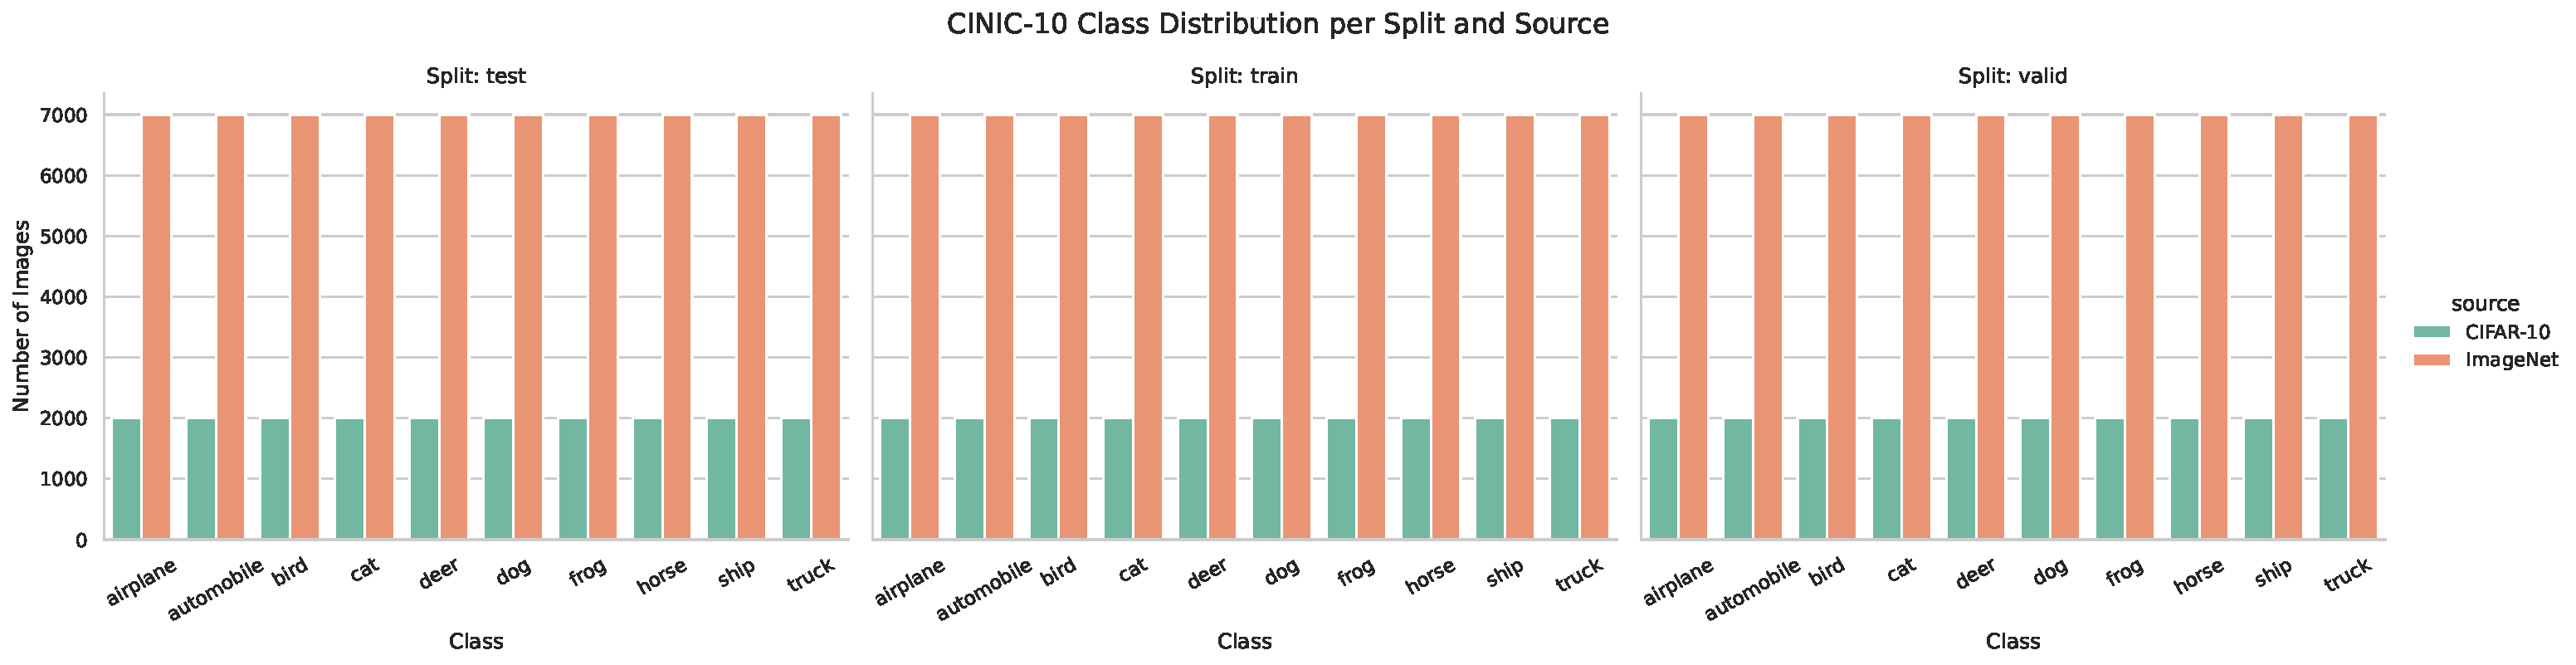
\includegraphics[width=0.95\textwidth]{Plots/DatasetOverview/cinic10_class_distribution.pdf}
    \caption{Distribution of classes and sources in the CINIC-10 dataset. Each class contains 9,000 images per split, but within each class, CIFAR-10 contributes 2,000 images and ImageNet 7,000.}
    \label{fig:class-distribution}
\end{figure}

In Figure~\ref{fig:rgb-stats}, we compare the mean and variance of RGB channel values per class, 
separated by source. While the differences appear small at first glance, they are systematic and consistent across categories. This suggests the 
presence of subtle domain-specific color or lighting distributions, which models might exploit when distinguishing between sources.

\begin{figure}[H]
    \centering
    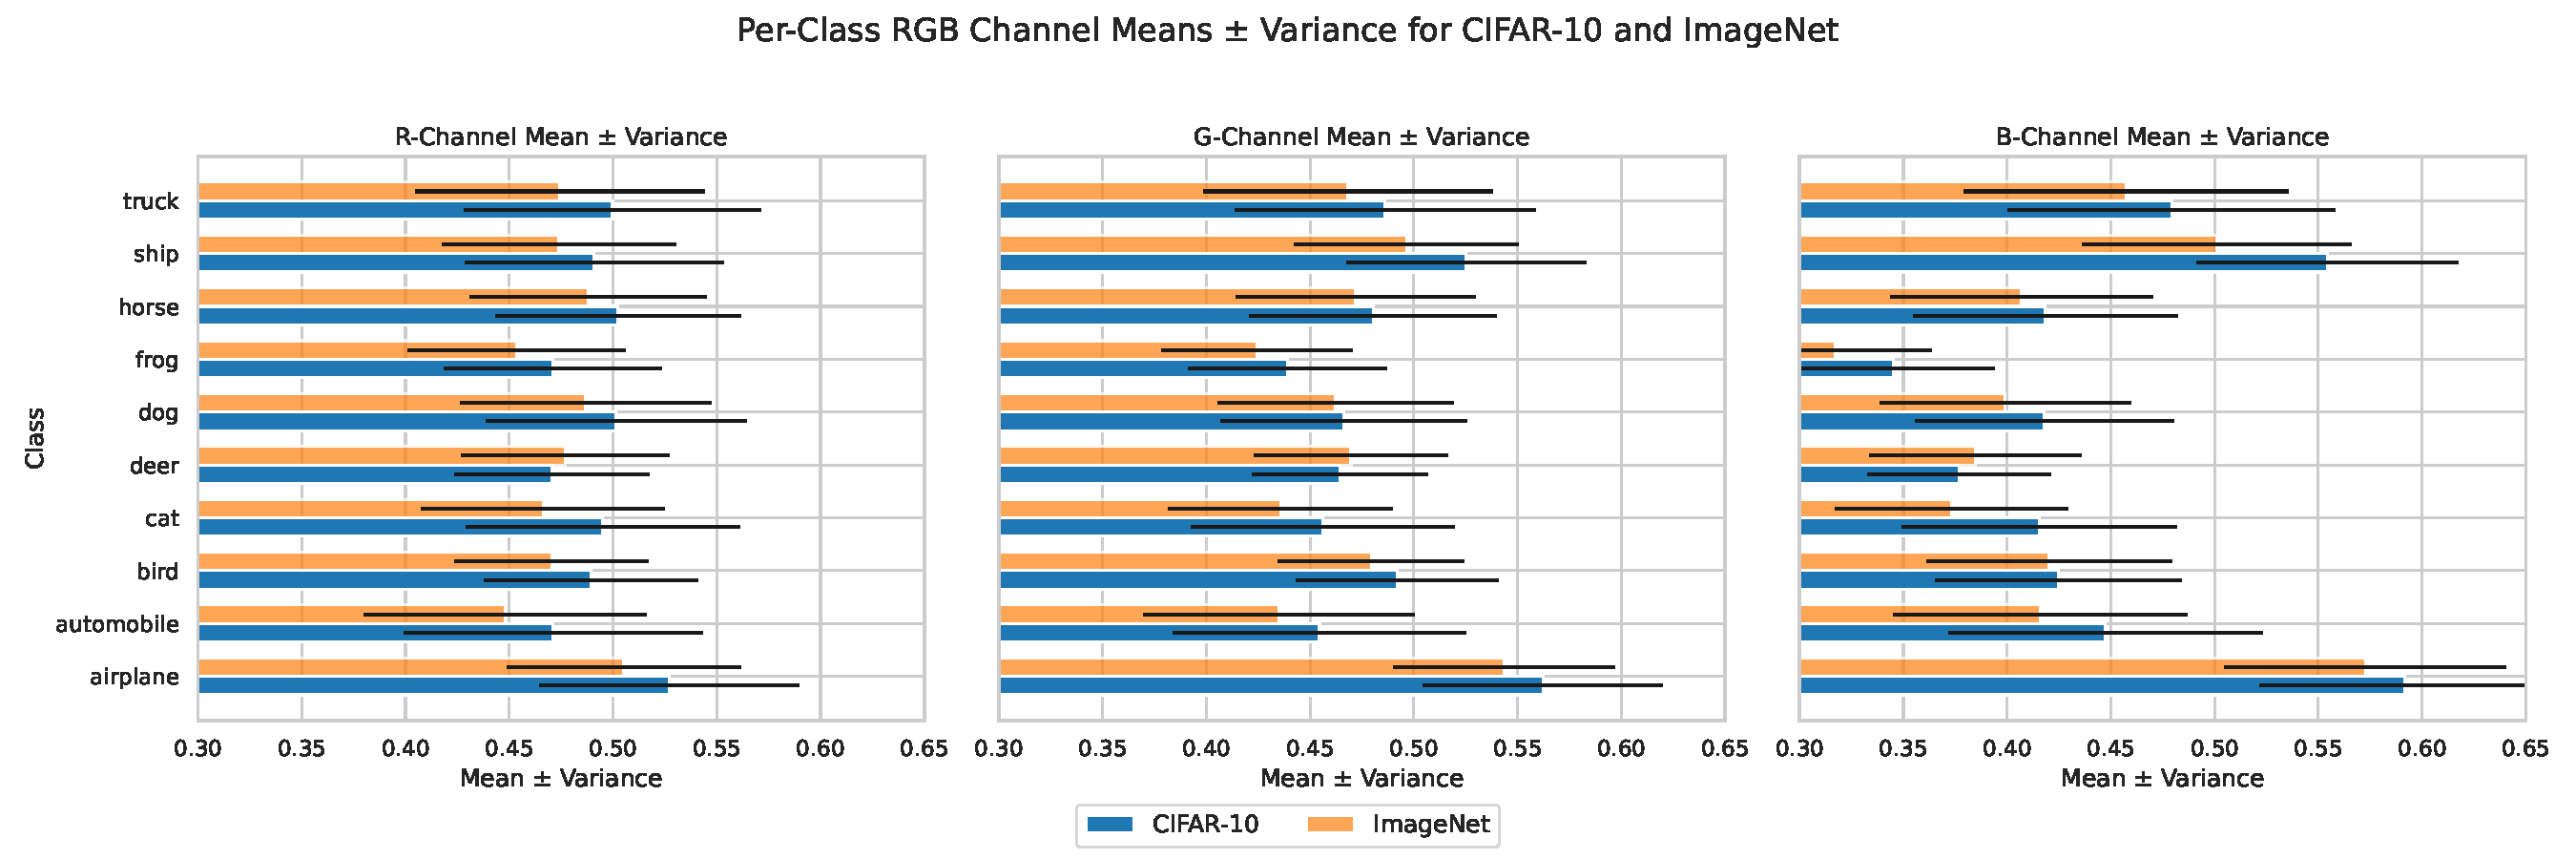
\includegraphics[width=0.95\textwidth]{Plots/DatasetOverview/rgb_means_variance_per_class.pdf}
    \caption{Mean and variance of RGB channels for each class, separated by source. Small but consistent differences between CIFAR-10 and ImageNet images are observable.}
    \label{fig:rgb-stats}
\end{figure}

To complement these quantitative statistics, we show concrete examples from the dataset. Figure~\ref{fig:automobile-comparison}
presents a comparison of the \textit{automobile} class from CIFAR-10 and ImageNet. CIFAR-10 images are visually uniform, typically centered and 
consistently lit. Imagenet appears to be mostly the same even though I can remember a remark at University that Cifar looks more "stockfootagy". 

To complement the quantitative results, we include visual examples from the dataset. Figure~\ref{fig:automobile-comparison} compares samples from the \textit{automobile} class in CIFAR-10 and ImageNet. While both sets feature centered and well-lit vehicles, CIFAR-10 images often appear more uniform and curated. This impression, sometimes likened to "stock footage," may partly result from prolonged exposure to similar, looking images during analysis.

Figure~\ref{fig:dog-comparison} shows examples from the \textit{dog} class. Again, CIFAR-10 
and ImageNet images appear to look simliar. Interestingly, the final image in the ImageNet row appears to be a 
fox, which highlights the presence of mislabeled or ambiguous samples in the dataset, as previously discussed by Northcutt et al.~\cite
{northcutt2021confident}.

\begin{figure}[H]
    \centering
    \begin{subfigure}[b]{\textwidth}
        \centering
        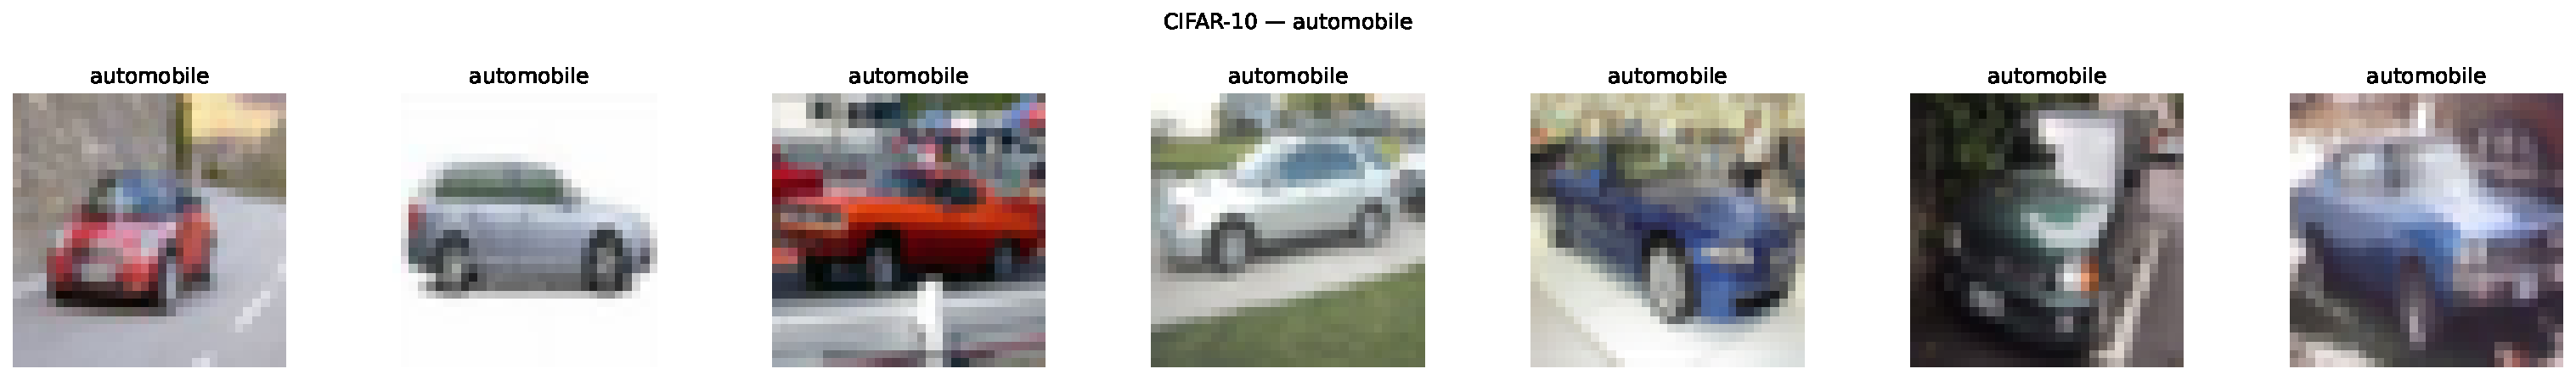
\includegraphics[width=\textwidth]{Plots/DatasetOverview/cifar_automobile_7_grid.pdf}
        \caption{CIFAR-10: \textit{automobile} class}
        \label{fig:cifar-automobile}
    \end{subfigure}

    \begin{subfigure}[b]{\textwidth}
        \centering
        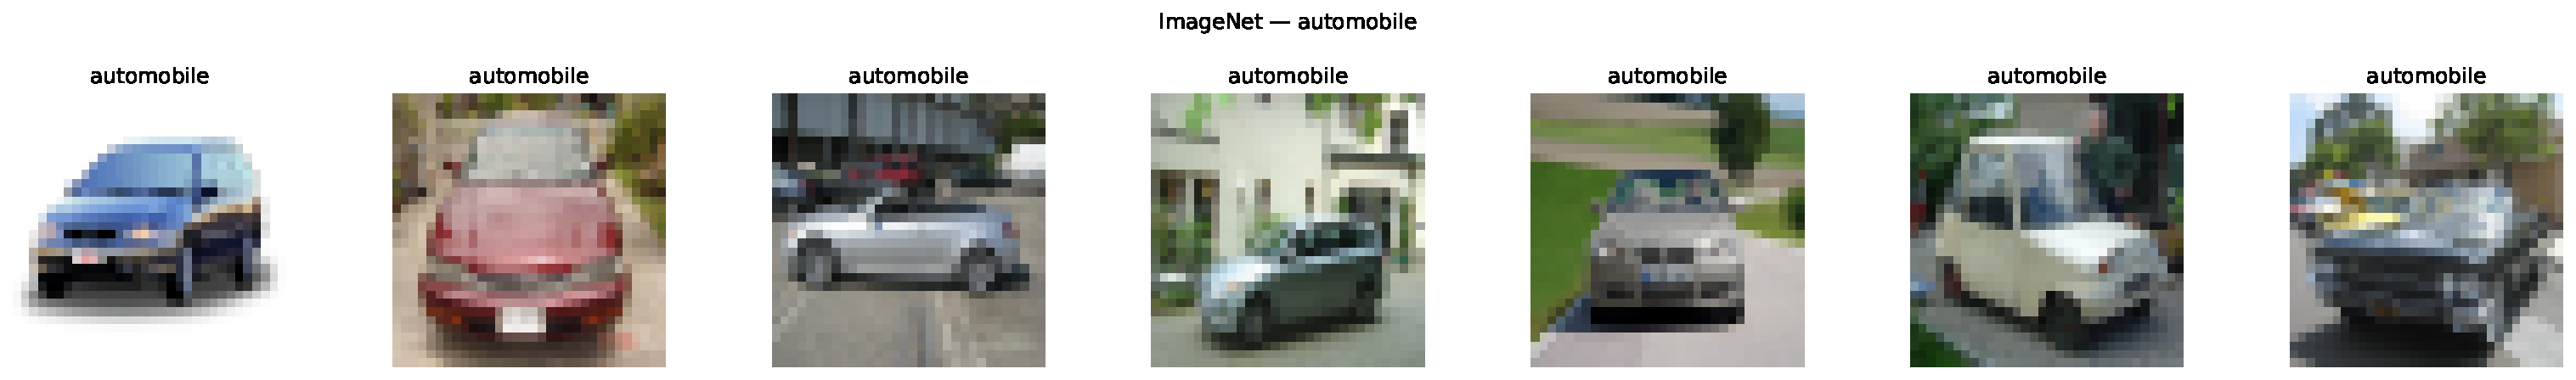
\includegraphics[width=\textwidth]{Plots/DatasetOverview/imageNet_automobile_7_grid.pdf}
        \caption{ImageNet: \textit{automobile} class}
        \label{fig:imagenet-automobile}
    \end{subfigure}
    
    \caption{Example images from the \textit{automobile} class in both CIFAR-10 and ImageNet.}
    \label{fig:automobile-comparison}
\end{figure}


\begin{figure}[H]
    \centering
    \begin{subfigure}[b]{\textwidth}
        \centering
        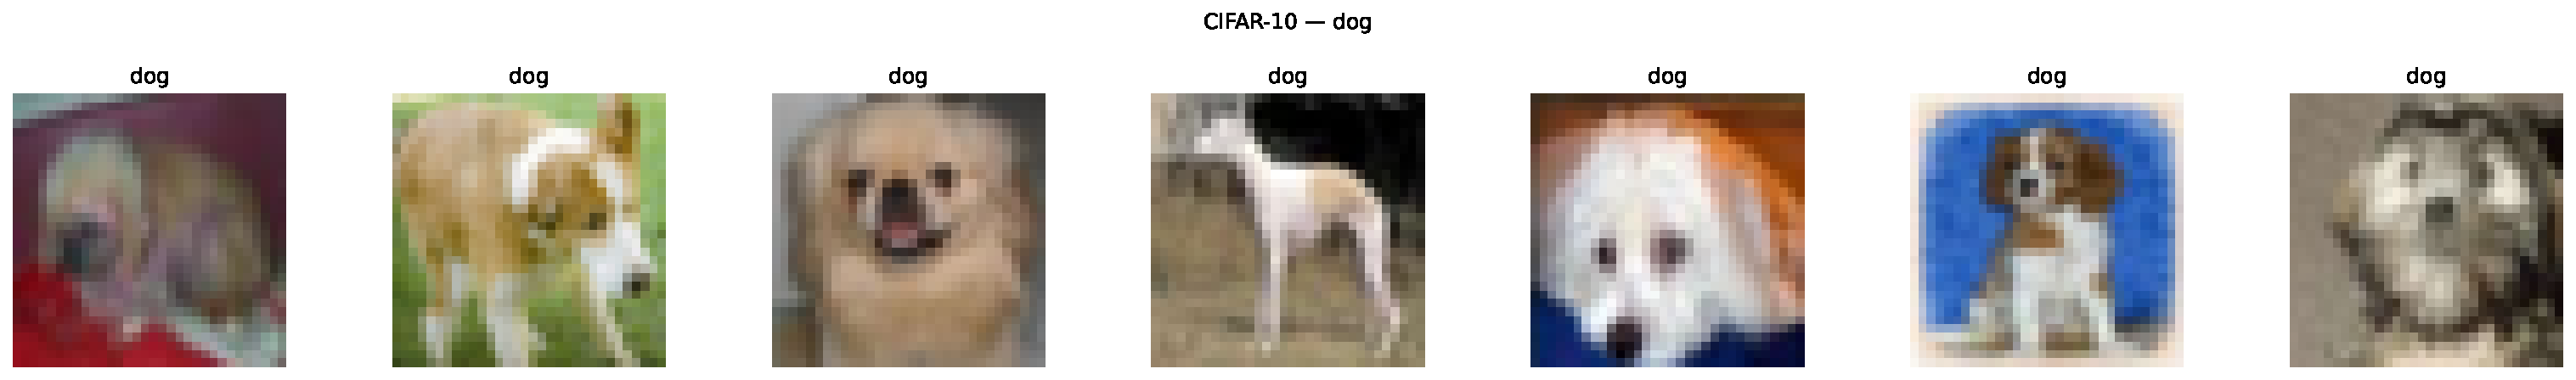
\includegraphics[width=\textwidth]{Plots/DatasetOverview/cifar_dog_7_grid.pdf}
        \caption{CIFAR-10: \textit{dog} class}
        \label{fig:cifar-dog}
    \end{subfigure}

    \begin{subfigure}[b]{\textwidth}
        \centering
        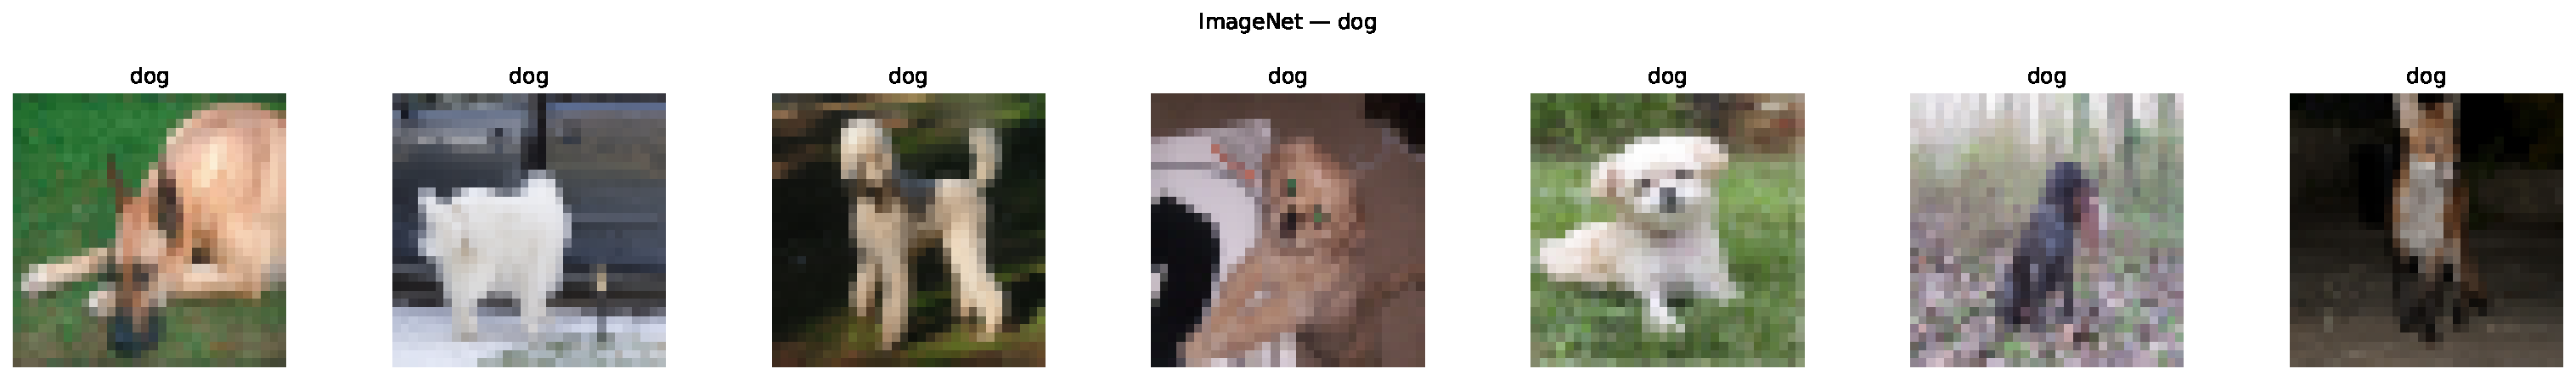
\includegraphics[width=\textwidth]{Plots/DatasetOverview/imageNet_dog_7_grid.pdf}
        \caption{ImageNet: \textit{dog} class}
        \label{fig:imagenet-dog}
    \end{subfigure}
    
    \caption{Example images from the \textit{dog} class in CIFAR-10 and ImageNet. Notably, the last ImageNet example appears to depict a fox, illustrating the presence of mislabeled data in the dataset as discussed in \cite{northcutt2021confident}.}
    \label{fig:dog-comparison}
\end{figure}

These visual and statistical comparisons highlight not only the domain differences between CIFAR-10 and ImageNet but also the types of cues a model 
might use to differentiate between them.

\section{Methodology}

This section describes the systematic approach we used to investigate whether a machine learning model can distinguish between CIFAR-10 and 
ImageNet images within the CINIC-10 dataset. Our methodology spans data preparation, model selection, training procedures and evaluation metrics.

\subsection{Problem Formulation}
We define the task as a binary classification problem: Given a $32 \times 32$ RGB image from the CINIC-10 dataset, can a model predict whether it 
originates from the CIFAR-10 or ImageNet domain, regardless of its class label? Each image is labeled with its source domain (0 for CIFAR-10, 1 for 
ImageNet), which serves as the prediction target.

\subsection{Data Preparation}
The details of the CINIC-10 dataset structure, class distribution and preprocessing steps are summarized in the \autoref{sec:Dataset Overview} (see Figures~\ref{fig:class-distribution} and~\ref{fig:automobile-comparison}). 
All data handling steps were based on the structure described there.

\subsection{Exploratory Statistical Analysis}
Before training models, we conducted an exploratory analysis of low level image statistics which is explained in \autoref{subsec:Examples and Visualizations}
(See Figure~\ref{fig:rgb-stats} for visualization).

\subsection{Model Architectures}
To evaluate the learnability of the source domain in CINIC-10, we trained a series of models with increasing complexity. We started with naive 
baselines, explored classical machine learning methods and ended with deep learning architectures.
To establish meaningful lower bounds, we implemented two simple baseline models and trained a Random Forest classifier using flattened image vectors
which served as a non-deep-learning benchmark.
As a neural baseline, we trained a fully connected model without convolutional layers.
We developed a minimal convolutional neural network using Keras to better capture spatial structure.
We visualized its learned kernels and activation maps to understand the spatial features it relied on. 
Subsequently, a slightly more complex model was trained, with hyperparameter optimization based on validation accuracy, 
to obtain a more realistic yet still lightweight architecture.
As a more advanced deep learning model, we trained a ResNet-18 architecture to evaluate how well a deep residual network can distinguish the domain origin.
This model serves as an upper bound in terms of complexity and performance. ResNet-18 hyperparameter optimization was omitted due to the model's already 
sufficient accuracy and the associated time complexity.


\subsection{Training Procedure}
\begin{itemize}
    \item The baseline models (Random Guessing, Majority Guessing, Random Forest) were trained using the combined \texttt{train} and \texttt{valid} splits.
    \item The rest of the models were trained on the \texttt{train} split and validated on the \texttt{valid} split.
    \item The final evaluation was performed on the separate \texttt{test} set for all models.
    \item Neural networks used the \texttt{Adam} optimizer with binary cross-entropy loss.
\end{itemize}

\subsection{Evaluation Metrics}
To evaluate model performance, we used the following metrics
\begin{itemize}
    \item \textbf{\texttt{classification\_report} from \texttt{scikit-learn}}: This provides precision, recall, F1-score and accuracy for each class \cite{scikit-learn}.
    \item \textbf{Confusion Matrix}: Used to visualize the classification performance and distinguish between CIFAR-10 and ImageNet predictions. We 
    employed the \texttt{heatmap} function from the \texttt{Seaborn} library for better readability and presentation \cite{Waskom2021}.
\end{itemize}
\section{Models and Results}
\label{sec:Models and Results}
This section presents a summary of each model's performance and includes key visualizations to illustrate their predictive capabilities.
A decision threshold of 0.5 was used for all models producing continuous predictions — i.e., predictions were classified as class 1 if the output 
was greater than 0.5, and as class 0 otherwise.

\subsection{Baselines: Random and Majority Guessing}

As a baseline, we implemented two trivial classifiers:

\begin{itemize}
    \item \textbf{Random Guessing}: Each image was randomly labeled as either \texttt{CIFAR-10} or \texttt{ImageNet} with 50\% probability. Over 100 runs, this yielded a mean accuracy of approximately \textbf{50\%}.
    \item \textbf{Majority Guessing}: Always predicting the dominant class (\texttt{ImageNet}) led to a test accuracy of \textbf{78\%}.
\end{itemize}

These baselines confirm that a high accuracy can be misleading in imbalanced datasets, emphasizing the need for more informative metrics.

\subsection{Random Forest Classifier}

Our non-deep learning benchmark was built using scikit-learn's \texttt{RandomForestClassifier}. We tested all combinations of the parameters 
\texttt{n\_estimators} (100, 150), \texttt{max\_depth} (None, 10, 20), \texttt{min\_samples\_split} (2, 5, 10), \texttt{max\_features} (\texttt{sqrt}, \texttt{log2}), 
and \texttt{criterion} (\texttt{gini}, \texttt{entropy}, \texttt{log\_loss}). The best performing model achieved an accuracy of \textbf{78.53\%}, 
which is again close to majority guessing. It predicted \texttt{ImageNet} in 89,188 out of 90,000 cases, thus strongly favouring the \texttt{ImageNet} domain.

%Our non-deep learning benchmark, was build using scikit-learn's \texttt{RandomForestClassifier}.
%Using the parameter candidates
%\begin{itemize}
%    \item \texttt{n\_estimators}: 100, 150
%    \item \texttt{max\_depth}: None, 10, 20
%    \item \texttt{min\_samples\_split}: 2, 5, 10
%    \item \texttt{max\_features}: \texttt{sqrt}, \texttt{log2}
%    \item \texttt{criterion}: \texttt{gini}, \texttt{entropy}, \texttt{log\_loss}
%\end{itemize}
%we created all possible parameter combinations.
%The best performing model achieved an accuracy of \textbf{78.53\%}, again close to majority guessing.
%It predicted \texttt{ImageNet} in 89,188 out of 90,000 cases thus strongly favouring \texttt{ImageNet}.

\subsection{Fully Connected Neural Network (MLP)}
The used MLP model used the architecture
\begin{itemize}
    \item Flatten → Dense(512, ReLU) → BatchNorm → Dropout(0.3)
    \item Dense(256, ReLU) → BatchNorm → Dropout(0.3)
    \item Dense(1, Sigmoid)
\end{itemize}
and reached a test accuracy of \textbf{78\%}, predicting \texttt{ImageNet} for 88,828 out of 90,000 test images. 
This again aligns with the majority baseline, showing that without spatial features, the model mostly learns the class imbalance.

\subsection{Minimal CNN for Visualization}
For interpretability, we trained a minimal convolutional network designed to extract and visualize learned kernels and feature maps:
\begin{itemize}
    \item Conv2D(2 filters)(3x3 Kernel) → MaxPooling2D → Flatten → Dense(1, Sigmoid)
\end{itemize}
Despite its simplicity, this model achieved a \textbf{96\%} test accuracy, with F1-scores of \textbf{0.91} for \texttt{CIFAR-10} and \textbf{0.97} for \texttt{ImageNet}. 
However, due to its limited use in drawing insights, we include its kernel and filtered image visualizations only in the 
Appendix~\ref{sec:Filter and Activation Visualizations — Minimal CNN}.

\newpage
\subsection{CNN with Hyperparameter Optimization}
We then developed a moderately complex (compared to the model before) CNN and optimized its hyperparameters using the optimization framework \texttt{Keras Tuner}~\cite{omalley2019kerastuner}. 

\setlength\intextsep{0pt}
\begin{wrapfigure}[12]{r}{0.5\textwidth}
    \begin{center}
        \vspace{-\baselineskip}
        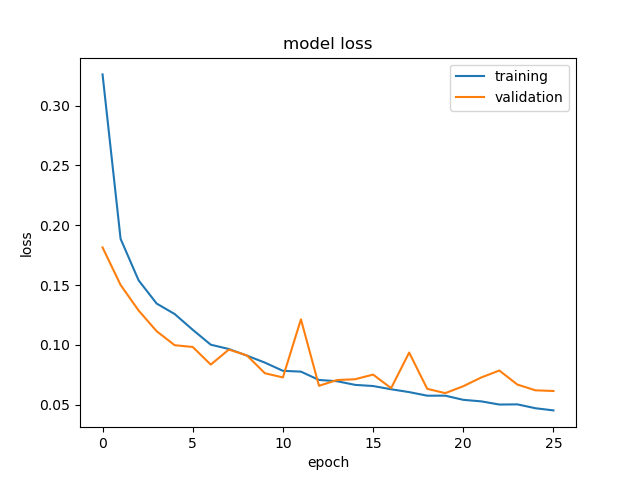
\includegraphics[width =0.48\textwidth]{Plots/ModelsAndResults/Hyperparameter_search_Loss.png}
        \caption{Training and validation loss of the CNN with Parameter ID P00.}
        \label{fig:hyperparameter_loss_plot}
    \end{center}
\end{wrapfigure}

The search space included Conv layer filter count and kernel size, use of a second Conv layer, Dropout rate, Dense layer units and the Learning rate.

Out of many configurations, the best CNN achieved the following on the test set
\begin{itemize}
    \item \textbf{Accuracy}: 98.19\%
    \item \textbf{F1-score (CIFAR-10)}: 0.96
    \item \textbf{F1-score (ImageNet)}: 0.99
\end{itemize}
and the training performance on the training and validation set over multiple epochs is shown in \autoref{fig:hyperparameter_loss_plot}.

To better understand how different hyperparameter configurations influenced the validation accuracy of our CNN model, 
\autoref{fig:Hyperparameter_Config_plot} visualizes the validation accuracy across tested configurations.
A sample of the configuration details is listed in \autoref{tab:Hyperparameter_Config_tab} in Appendix~\ref{sec:Hyperparameter Configurations}.

\begin{figure}[H]
    \centering
    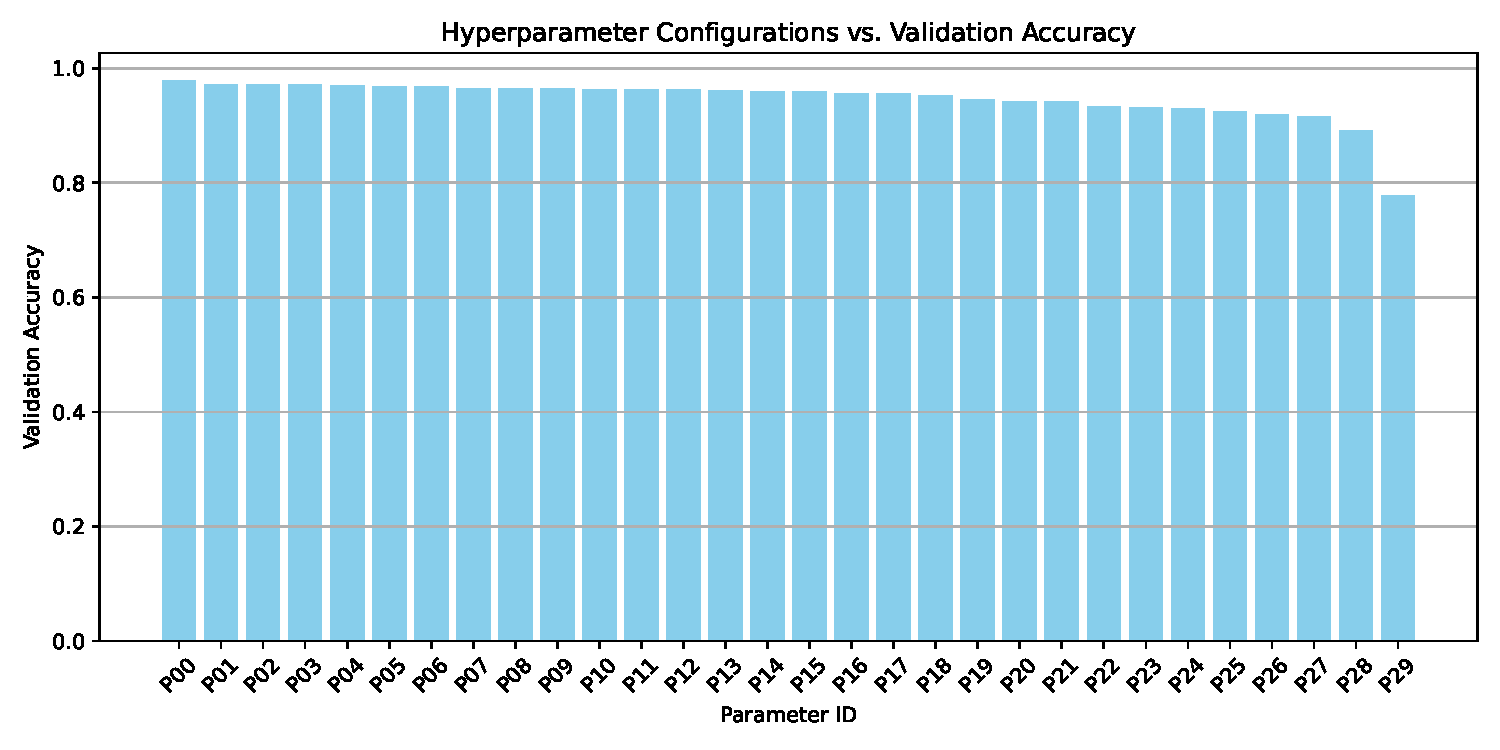
\includegraphics[width=0.9\textwidth]{Plots/ModelsAndResults/Hyperparameter_Config_plot.pdf}
    \caption{Validation accuracy for selected hyperparameter configurations tested with Keras Tuner. Each configuration ID corresponds to one model setup.}
    \label{fig:Hyperparameter_Config_plot}
\end{figure}

\raggedbottom
\addtolength{\topskip}{0pt plus 10pt}
This model demonstrated that with enough capacity and tuning, even modest CNNs can learn highly predictive domain-specific features.


\subsection{ResNet-18}

To evaluate how well a deeper architecture performs, we trained a \textbf{ResNet-18} model~\cite{he2016ResNet18} on the same binary classification task. 
Without any hyperparameter tuning, the model reached:

\begin{itemize}
    \item \textbf{Accuracy}: 99.26\%
    \item \textbf{F1-score (CIFAR-10)}: 0.98
    \item \textbf{F1-score (ImageNet)}: 1.00
\end{itemize}

\autoref{fig:ResNet18_loss_plot} illustrates the loss and validation performance over the training epochs, suggesting the models capabilities being bigger then needed.  
To further analyze performance, we include \autoref{fig:ResNet18_confusion_matrix_plot}, which presents the confusion matrix for test predictions. 
The nearly perfect separation between CIFAR-10 and ImageNet images supports the conclusion that this deep model can exploit source-specific characteristics with high reliability.

\begin{figure}[H]
    \centering
    \begin{subfigure}[b]{0.48\textwidth}
        \centering
        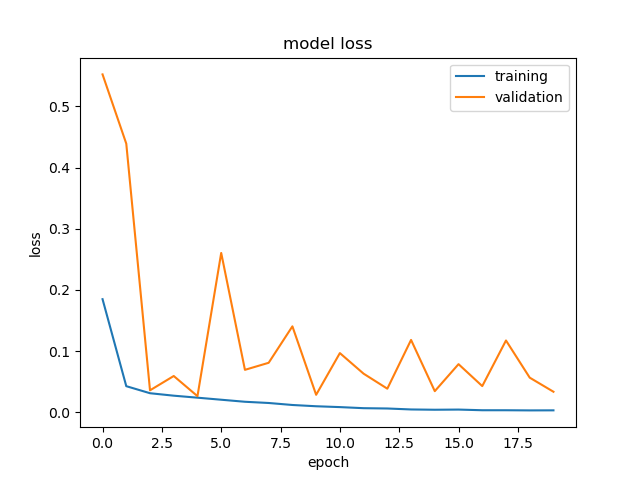
\includegraphics[width=\textwidth]{Plots/ModelsAndResults/ResNet18_Loss.png}
        \caption{Loss and validation accuracy of ResNet-18 during training.}
        \label{fig:ResNet18_loss_plot}
    \end{subfigure}
    \hfill
    \begin{subfigure}[b]{0.48\textwidth}
        \centering
        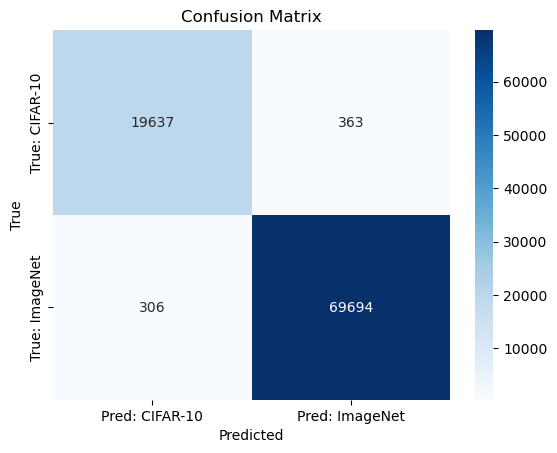
\includegraphics[width=\textwidth]{Plots/ModelsAndResults/ResNet18_confusion_matrix.png}
        \caption{Confusion matrix of ResNet-18 predictions on the test data.}
        \label{fig:ResNet18_confusion_matrix_plot}
    \end{subfigure}
    \caption{Training behavior and evaluation of ResNet-18 model.}
    \label{fig:ResNet18_combined}
\end{figure}

These results confirm that deep architectures like ResNet-18 can achieve near-perfect source discrimination, setting a strong upper performance bound for this task. \newpage
% \section{Discussion}
%Our experiments confirm that the CINIC-10 dataset exhibits strong source-identifiable features. Even relatively simple models were able to 
%distinguish between CIFAR-10 and ImageNet images with high accuracy. The Random Forest classifier, trained on flattened pixel data, achieved nearly 
%the same accuracy as a majority-guessing baseline, predicting ImageNet in over 89,000 out of 90,000 test cases. This suggests that the 
%distinguishability between the two sources relies heavily on two-dimensional spatial structures rather than just global pixel statistics. Despite 
%all images having identical dimensions and class labels, the hypothesis that the two sources differ in their visual characteristics can still be 
%answered affirmatively, as supported by the accuracy results presented in \autoref{sec:Models and Results}.
%
%More powerful models, including convolutional neural networks and a ResNet-18, further demonstrated the learnability of the domain source. The 
%ResNet-18 achieved a test accuracy of 99.26\%, indicating that structural cues in the image data make the source label trivially learnable when 
%using deep models. This confirms the domain shift inherent in the CINIC-10 construction and underscores the need for domain adaptation strategies 
%when applying such datasets in real-world settings due to image predictions need to be not reliant on domain.
%
%More powerful models, including convolutional neural networks and a ResNet-18, further demonstrated the ease with which the source domain can be 
%learned. The ResNet-18 model achieved a test accuracy of 99.26\%, highlighting that structural cues in the image data make the source label 
%predictable for deep learning models. This confirms the presence of a domain shift in the CINIC-10 dataset and underscores the importance of domain 
%adaptation techniques in real-world applications, where model predictions should not rely on superficial domain-specific features.
%
%To investigate the impact of resolution artifacts introduced during dataset construction, we explored upscaling and downscaling techniques. Following the 
%approach outlined in the CINIC-10 GitHub repository \cite{cinic10_github}, we rescaled images using the same downsampling algorithm used to generate the dataset.
%We tested various combinations: upscaling and downscaling only CIFAR-10 images, only ImageNet images and both. We trained models on original (non-rescaled) 
%images and evaluated performance when test images were rescaled accordingly.
%
%Interestingly, training models on both scaled and non-scaled images did not prevent learning, although it slowed convergence slightly in the case 
%of minimal CNNs. More surprisingly, rescaling only the CIFAR-10 test images led to a slight improved classification performance, while rescaling 
%ImageNet images resulted in a significantly reduced accuracy. This contradicts our expectation that CIFAR-10 images, after being upscaled, would 
%resemble ImageNet images more closely and thus be misclassified as such. Instead, the models became more confident in identifying CIFAR-10. Due to 
%time constraints, we were unable to fully explore this unexpected asymmetry, but it suggests that the interpolation artifacts introduced by 
%rescaling might make CIFAR-10 images more distinguishable rather than less.
%
%Another avenue we explored involved visualizing learned filters of a minimal CNN model. Despite achieving high accuracy (96\%) and favorable 
%F1-scores (0.91 for CIFAR-10 and 0.97 for ImageNet), these visualizations yielded little interpretative value, suggesting that simple models may 
%rely on subtle cues that are not easily visualized. Filter visualizations for this minimal network are included in Appendix~\ref{sec:Filter and 
%Activation Visualizations — Minimal CNN}.
%
%Overall, our findings highlight that even in a dataset constructed to balance classes and resolution, the underlying data distributions remain 
%distinguishable by source. This raises concerns for any supervised learning task that assumes dataset homogeneity. While deeper models can exploit 
%these domain cues to achieve near-perfect classification, such performance may be misleading in applications where the source domain should be 
%irrelevant.
%
%Our results demonstrate that, although CIFAR-10 and ImageNet images may not appear easily distinguishable to the human eye—a claim that could be 
%validated through user studies—underlying differences between the source domains remain highly learnable. This presents a challenge for supervised 
%learning tasks that assume domain invariance. Deep models, in particular, can exploit subtle domain-specific signals to achieve high performance. 
%However, such results may be misleading in applications where the source of the data should play no role in the prediction. These findings 
%highlight the importance of careful dataset construction and the need for domain adaptation strategies when deploying models in heterogeneous or 
%cross-domain settings.

% The discussion above is to long and this below uses chat gpt to summarize and shorten so i stay within my page limits :)
\section{Discussion}

Our experiments show that the CINIC-10 dataset contains strong source identifiable signals. Even simple models could reliably tell apart CIFAR-10 
and ImageNet images. The Random Forest classifier and Dense Neural Network, trained on flattened pixels, performed close to a majority baseline and 
heavily favored predicting ImageNet. This suggests that the differences between the two domains rely on spatial structures rather than just basic 
statistics.

More complex models, such as CNNs and ResNet-18, were able to separate the domains almost perfectly. The ResNet-18 model reached 99.26\% accuracy, 
highlighting how easily deep networks can pick up on structural cues tied to the image source. This confirms the presence of domain shift in 
CINIC-10 and raises concerns for tasks where domain independence is important.

To explore how scaling affects model performance, we tried upscaling and downscaling the CIFAR-10 and ImageNet images using the same method 
described in the CINIC-10 repository~\cite{cinic10_github}. We tested multiple scenarios: rescaling only one of the domains, both or none. 
Training on mixed scaled and non-scaled data was still effective, though convergence slowed for small CNNs. Surprisingly for models trained on the 
normal dataset and up- and down- scaling only the CIFAR-10 test images slightly improved performance, while rescaling ImageNet images reduced 
accuracy. We had expected the opposite effect. This unexpected result suggests that interpolation artifacts might have made CIFAR-10 images more 
easily identifiable. Further testing is needed to understand this better and was not included in the main part of this report due to insufficient testing.

We also visualized filters from a minimal CNN model that achieved 96\% accuracy. However, the visualizations offered limited insight, suggesting 
that the model relied on subtle differences not easily interpreted. These are included in 
Appendix~\ref{sec:Filter and Activation Visualizations — Minimal CNN}.

Even though CIFAR-10 and ImageNet images appear visually similar, models clearly learn to distinguish them. This challenges the assumption that 
combining datasets with matching resolution and labels removes domain specific cues. It underlines the importance of domain adaptation techniques 
and careful dataset design for fair and reliable model training. \newpage
%\section{Conclusion and Future Work}
%
%This work examined the domain identifiability of the CINIC-10 dataset, which merges CIFAR-10 and downsampled ImageNet images into a single 
%benchmark. Although the two sources share class labels and image resolution, our experiments revealed that even simple models can reliably identify 
%the source of an image. More powerful models, including a ResNet-18, achieved near-perfect accuracy by leveraging structural cues inherent in the 
%data.
%
%These findings indicate that CINIC-10 retains source specific characteristics to an extent that allows models to easily separate the domains. This 
%raises concerns for using CINIC-10 in tasks that assume domain invariance and highlights the importance of thorough dataset evaluation, especially 
%in the context of transfer learning, fairness, and domain generalization.
%
%\subsection*{Future Work}
%
%Several promising directions remain for future investigation:
%
%\begin{itemize}
%    \item \textbf{Human evaluation}: It would be interesting to test whether people can tell apart CIFAR-10 and ImageNet images. This could help 
%    assess whether the domain differences exploited by models are also perceptible to humans.
%
%    \item \textbf{Other dataset combinations}: Similar experiments could be done with other merged datasets—like combining CIFAR-10 with STL-10 or 
%    using subsets of Tiny ImageNet—to see whether such domain differences are common or specific to CINIC-10.
%
%    \item \textbf{Asymmetric scaling strategies}: Instead of downscaling both datasets the same way, one could try upscaling CIFAR-10 images 
%    slightly and only downscale ImageNet images once (instead of reducing them too aggressively). This might help equalize their visual 
%    characteristics without heavily degrading one side.
%
%    \item \textbf{Domain adaptation techniques}: Methods like domain-adversarial training, style transfer, or aligning feature distributions could 
%    be used to reduce the model's reliance on domain-specific cues and shift its focus toward more meaningful features.
%
%    \item \textbf{Model interpretation}: To better understand how models make their decisions, one could apply explainability tools like saliency 
%    maps or SHAP values to identify which image regions contribute most to source predictions.
%\end{itemize}
%
%Ultimately, our findings highlight the importance of careful dataset design and evaluation, especially in contexts where fairness, robustness, or 
%generalization across domains plays a critical role.

% The Conclusion and Future Work above is to long and this below uses chat gpt to summarize and shorten so i stay within my page limits :)
\section{Conclusion and Future Work}

This work explored how easily the source domain of images in CINIC-10 can be learned. Despite having the same resolution and class labels, 
models, ranging from simple baselines to a ResNet-18, were able to distinguish CIFAR-10 and ImageNet samples with high accuracy. This shows that 
CINIC-10 preserves domain specific signals, which can mislead performance assessments in tasks that assume domain invariance.

To build on this, future work could involve testing whether humans can also tell the sources apart, or repeating the experiments with other 
combined datasets like CIFAR-10 and STL-10. Another interesting direction would be to experiment with asymmetric scaling strategies, such as 
upscaling CIFAR-10 and only lightly downscaling ImageNet, to reduce domain cues. Techniques like adversarial domain adaptation or feature alignment 
could help models focus on class relevant features instead. Finally, interpreting model behavior using tools like saliency maps or SHAP values 
could offer deeper insights into what cues are being used for source prediction.

In short, this study underscores the importance of evaluating dataset construction and model behavior, especially when generalization, fairness, or 
robustness matter. \newpage


% APPENDIX
% Hier beginnt der Anhang, nummeriert in lateinischen Buchstaben
\appendix
\newpage
\renewcommand{\thesection}{\Alph{section}}  % A, B, C...

\section{Further Reading}
\label{sec:further-reading}

For readers seeking a gentle introduction to the core concepts of machine learning referenced in this report, we recommend the following resources:

\begin{itemize}
  \item \textbf{Neural Networks and Deep Learning (Michael Nielsen)} \newline
  An excellent interactive online book introducing neural networks from scratch.  \newline
  \url{http://neuralnetworksanddeeplearning.com/}  
  
  \item \textbf{Google's Machine Learning Crash Course}  \newline
  A practical introduction to ML with TensorFlow, including video lectures and exercises.  \newline
  \url{https://developers.google.com/machine-learning/crash-course}

  \item \textbf{3Blue1Brown: Neural Networks Series (YouTube)}  \newline
  Visually intuitive explanations of neural networks and backpropagation.  \newline
  \url{https://shorturl.at/oQq8L}
  
  \item \textbf{Scikit-learn Documentation: Decision Trees and Random Forests}  \newline
  Concise explanations of the implementation method for random Forests used in this Report.  \newline
  \url{https://scikit-learn.org/stable/modules/ensemble.html}
  
  \item \textbf{Distill.pub: Feature Visualization}  \newline
  For understanding what deep neural networks “see.”  \newline
  \url{https://distill.pub/2017/feature-visualization/}
\end{itemize} \newpage
\section{Filter and Activation Visualizations — Minimal CNN}
\label{sec:Filter and Activation Visualizations — Minimal CNN}

 \newpage
\section{Hyperparameter Configurations}
\label{sec:Hyperparameter Configurations}

% \begin{table}[H]
%     \centering
%     \caption{Ten out of 30 selected hyperparameter configurations explored during model tuning with Keras Tuner. Each configuration specifies 
%     convolutional filter sizes and kernel dimensions of the first convolution Layer, dropout rates (DR), dense layer size (DU = Dense Units), 
%     learning rate, and whether a second convolutional layer was used an its corresponding Filter number and Kernel size. 
%     These settings were evaluated to optimize validation accuracy.}
%     \label{tab:Hyperparameter_Config_tab}
%     \begin{tabular}{lrrlrrrrr}
%         \hline
%         \textbf{ID} & \textbf{Filt. 1} & \textbf{Kern. 1} & \textbf{Conv 2} & \textbf{DR} & \textbf{DU} & \textbf{LR} & 
%         \textbf{Filt. 2} & \textbf{Kern. 2} \\
%         \hline
%         P00 & 40 & 3 & True  & 0.2 & 128 & 0.00034 & 40 & 3 \\
%         P01 & 16 & 3 & True  & 0.2 & 48  & 0.00023 & 40 & 3 \\
%         P02 & 56 & 3 & False & 0.2 & 96  & 0.00060 &    &   \\
%         P03 & 16 & 3 & True  & 0.1 & 64  & 0.00051 & 32 & 3 \\
%         P04 & 40 & 3 & True  & 0.2 & 128 & 0.00034 & 40 & 3 \\
%         P05 & 32 & 5 & True  & 0.3 & 96  & 0.00142 & 48 & 5 \\
%         P06 & 56 & 3 & False & 0.2 & 96  & 0.00060 &    &   \\
%         P07 & 8  & 5 & True  & 0.4 & 48  & 0.00018 & 8  & 3 \\
%         P08 & 40 & 3 & False & 0.3 & 16  & 0.00156 &    &   \\
%         P09 & 16 & 3 & True  & 0.5 & 80  & 0.00074 & 16 & 5 \\
%         \hline
%     \end{tabular}
% \end{table}

\begin{table}[H]
    \centering
    \caption{All 30 selected hyperparameter configurations explored during model tuning with Keras Tuner. Each configuration specifies 
    convolutional filter sizes and kernel dimensions of the first convolution layer, dropout rates (DR), dense layer size (DU~=~Dense~Units), 
    learning rate and whether a second convolutional layer was used and its corresponding filter number and kernel size. 
    These settings were evaluated to optimize validation accuracy.}
    \label{tab:Hyperparameter_Config_tab}
    \begin{tabular}{lrrlrrrrr}
        \hline
        \textbf{ID} & \textbf{Filt. 1} & \textbf{Kern. 1} & \textbf{Conv 2} & \textbf{Filt. 2} & \textbf{Kern. 2} 
        & \textbf{DR} & \textbf{DU} & \textbf{LR} \\
        \hline
        P00 & 40 & 3 & True  & 40 & 3 & 0.2 & 128 & 0.00034 \\
        P01 & 16 & 3 & True  & 40 & 3 & 0.2 & 48  & 0.00023 \\
        P02 & 56 & 3 & False &    &   & 0.2 & 96  & 0.00060 \\
        P03 & 16 & 3 & True  & 32 & 3 & 0.1 & 64  & 0.00051 \\
        P04 & 40 & 3 & True  & 40 & 3 & 0.2 & 128 & 0.00034 \\
        P05 & 32 & 5 & True  & 48 & 5 & 0.3 & 96  & 0.00142 \\
        P06 & 56 & 3 & False &    &   & 0.2 & 96  & 0.00060 \\
        P07 & 8  & 5 & True  & 8  & 3 & 0.4 & 48  & 0.00018 \\
        P08 & 40 & 3 & False &    &   & 0.3 & 16  & 0.00156 \\
        P09 & 16 & 3 & True  & 16 & 5 & 0.5 & 80  & 0.00074 \\
        P10 & 40 & 3 & False &    &   & 0.5 & 80  & 0.00398 \\
        P11 & 40 & 3 & False &    &   & 0.5 & 80  & 0.00398 \\
        P12 & 40 & 3 & False &    &   & 0.3 & 16  & 0.00156 \\
        P13 & 40 & 3 & False &    &   & 0.5 & 32  & 0.00126 \\
        P14 & 56 & 5 & False &    &   & 0.3 & 32  & 0.00059 \\
        P15 & 64 & 5 & False &    &   & 0.2 & 112 & 0.00012 \\
        P16 & 32 & 3 & False &    &   & 0.1 & 48  & 0.00037 \\
        P17 & 16 & 5 & False &    &   & 0.4 & 112 & 0.00068 \\
        P18 & 40 & 3 & False &    &   & 0.3 & 16  & 0.00156 \\
        P19 & 56 & 3 & False &    &   & 0.2 & 96  & 0.00060 \\
        P20 & 16 & 3 & True  & 16 & 5 & 0.5 & 80  & 0.00074 \\
        P21 & 40 & 3 & False &    &   & 0.5 & 32  & 0.00126 \\
        P22 & 40 & 5 & False &    &   & 0.2 & 80  & 0.00140 \\
        P23 & 24 & 5 & True  & 8  & 3 & 0.3 & 112 & 0.00023 \\
        P24 & 64 & 3 & False &    &   & 0.1 & 80  & 0.00014 \\
        P25 & 48 & 3 & False &    &   & 0.2 & 16  & 0.00061 \\
        P26 & 48 & 3 & False &    &   & 0.1 & 32  & 0.00021 \\
        P27 & 24 & 5 & False &    &   & 0.5 & 64  & 0.00299 \\
        P28 & 32 & 3 & True  & 8  & 5 & 0.5 & 112 & 0.00483 \\
        P29 & 24 & 5 & False &    &   & 0.3 & 96  & 0.00614 \\
        \hline
    \end{tabular}
\end{table}
 \newpage

%\backmatter
\printbibliography

\cleardoublepage
% From https://www.tu-dortmund.de/studierende/im-studium/pruefungsangelegenheiten/allgemeine-vordrucke/
% 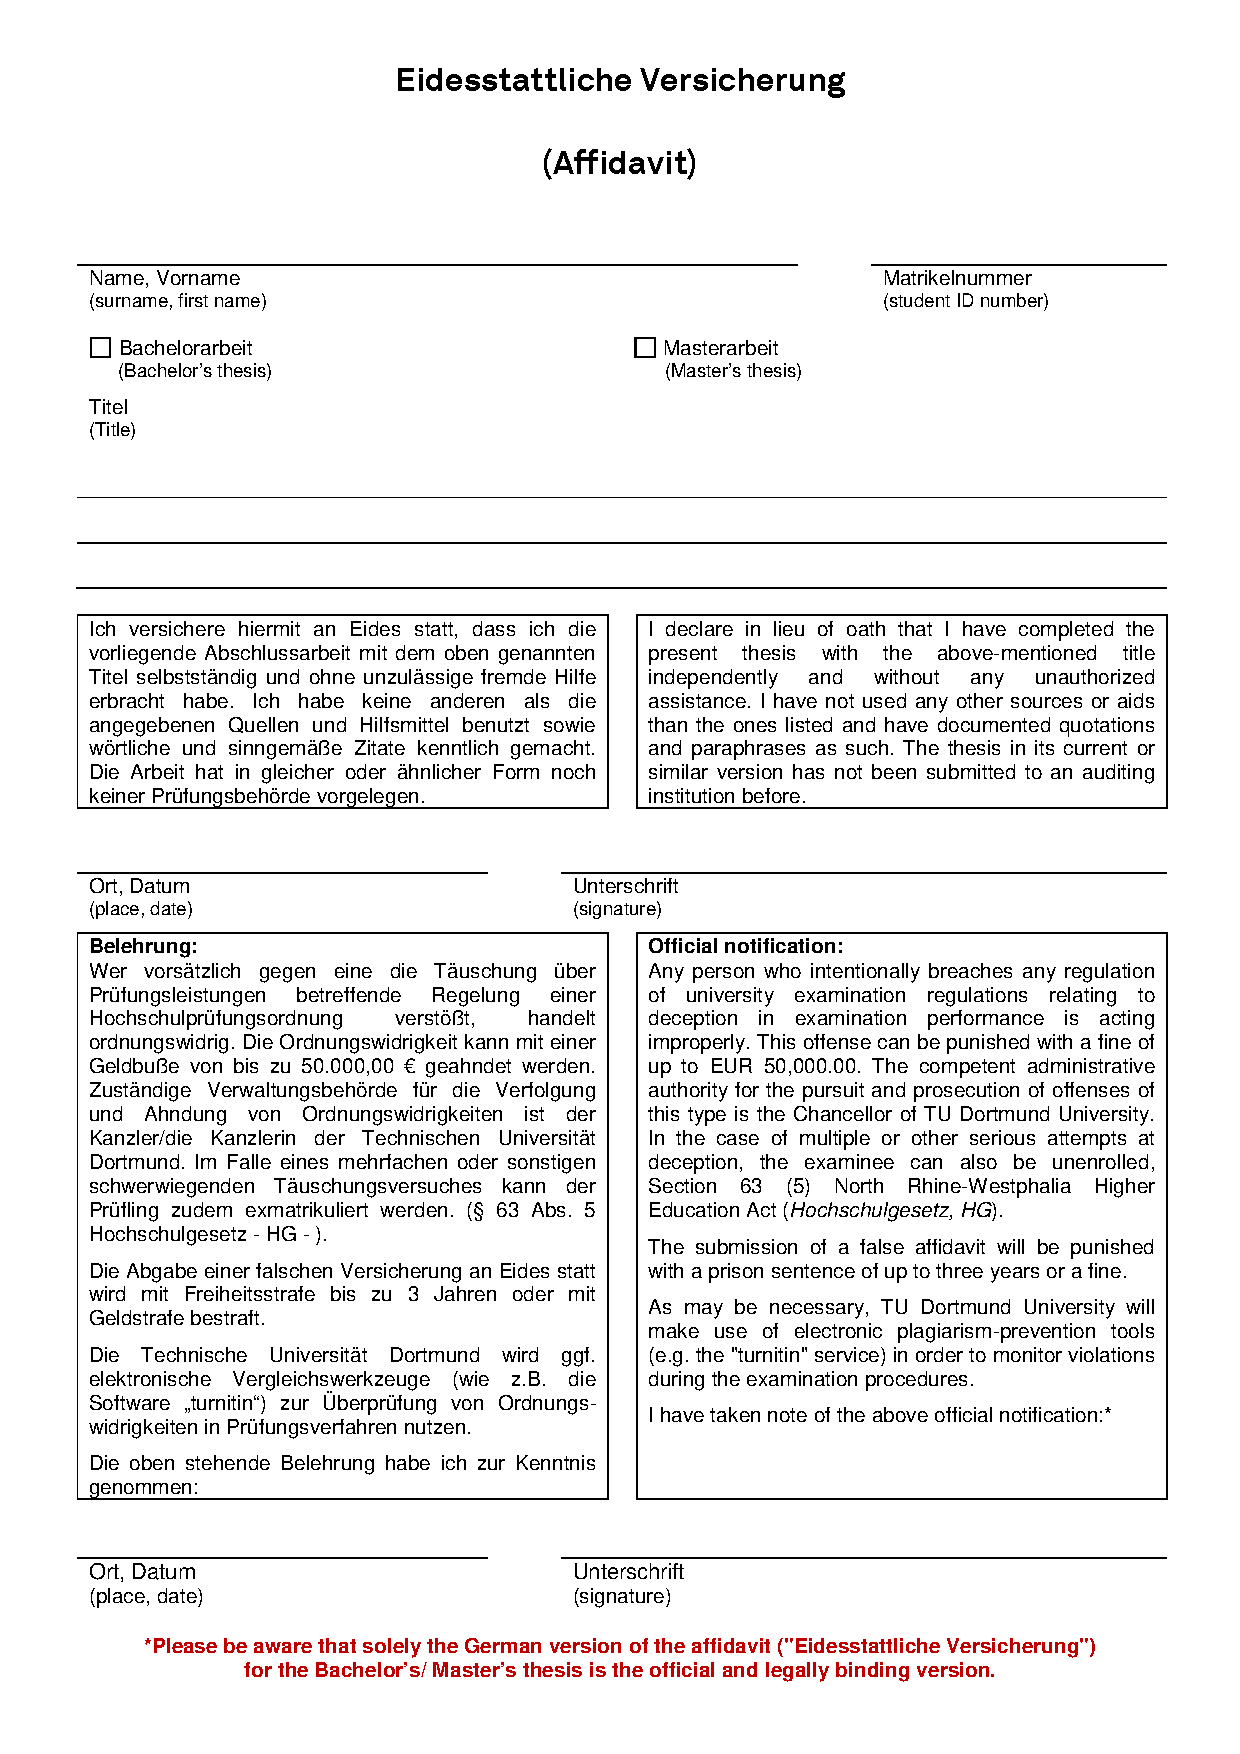
\includepdf{content/Eidesstattliche_Versicherung.pdf}

\end{document}
